\documentclass[11pt,a4paper]{article}

\usepackage[dvipsnames]{xcolor}

\newcommand{\teamname}{Binary}
\newcommand{\topicchoice}{Topic 4 -- Async Research Assistant}
\newcommand{\reportdate}{July 27, 2026}
\newcommand{\repolink}{\url{https://github.com/mrorxan/research-assistant}}

\newcommand{\coursecode}{AI-ENG-110}
\newcommand{\coursename}{Software Engineering}
\newcommand{\institution}{AI Academy, National AI Center}
\newcommand{\semester}{Spring 2026}

\usepackage[margin=2.2cm,headheight=15pt]{geometry}
\usepackage[T1]{fontenc}
\usepackage[utf8]{inputenc}
\usepackage[final,protrusion=true,expansion=false]{microtype}
\usepackage{amsmath,amssymb}
\usepackage{graphicx}
\usepackage{booktabs}
\usepackage{array}
\usepackage{tabularx}
\usepackage{ragged2e}
\usepackage{enumitem}
\usepackage[parfill]{parskip}
\usepackage{listings}
\usepackage{tikz}
\usetikzlibrary{shapes.geometric,arrows.meta,positioning}
\usepackage{titlesec}
\usepackage{fancyhdr}
\usepackage{lastpage}
\usepackage[hidelinks]{hyperref}

\emergencystretch=3em
\hbadness=10000
\hfuzz=2pt

\hypersetup{
  colorlinks=true,
  linkcolor=NavyBlue,
  urlcolor=NavyBlue,
  citecolor=NavyBlue,
  pdftitle={\coursecode\ Final Project Report},
  pdfauthor={\teamname}
}

\definecolor{accent}{HTML}{0B3D91}
\definecolor{soft}{HTML}{F2F4F8}
\definecolor{ok}{HTML}{166534}

\titleformat{\section}
  {\Large\bfseries\color{accent}}{\thesection.}{0.6em}{}
\titleformat{\subsection}
  {\large\bfseries\color{accent}}{\thesubsection}{0.5em}{}

\definecolor{codegreen}{rgb}{0,0.55,0}
\definecolor{codegray}{rgb}{0.4,0.4,0.4}
\definecolor{codepurple}{rgb}{0.55,0,0.78}
\definecolor{backcolour}{rgb}{0.97,0.97,0.97}

\lstdefinestyle{python}{
  language=Python,
  backgroundcolor=\color{backcolour},
  commentstyle=\color{codegreen},
  keywordstyle=\color{accent},
  numberstyle=\tiny\color{codegray},
  stringstyle=\color{codepurple},
  basicstyle=\ttfamily\footnotesize,
  breakatwhitespace=false,
  breaklines=true,
  keepspaces=true,
  showstringspaces=false,
  numbers=left,
  numbersep=6pt,
  tabsize=2,
  frame=single,
  framerule=0.4pt,
  rulecolor=\color{black!30},
}

\pagestyle{fancy}
\fancyhf{}
\fancyhead[L]{\small\textit{\coursecode\ -- Final Report -- \teamname}}
\fancyhead[R]{\small\textit{\semester}}
\fancyfoot[L]{\small\textit{\institution}}
\fancyfoot[R]{\small Page \thepage\ of \pageref{LastPage}}
\renewcommand{\headrulewidth}{0.4pt}
\renewcommand{\footrulewidth}{0.4pt}

\begin{document}

\begin{center}
{\small \textsc{\institution} \\[0.2em] \textsc{\coursecode\ -- \coursename\ -- \semester}}\\[1.2em]
{\Large\bfseries\color{accent} Final Project Report}\\[0.3em]
{\LARGE\bfseries \topicchoice}\\[0.6em]
\rule{0.85\textwidth}{0.6pt}
\end{center}

\vspace{0.6em}
\begin{tabularx}{\textwidth}{@{}lXlX@{}}
\textbf{Team:} & \teamname & \textbf{Date:} & \reportdate \\
\textbf{Repo:} & \repolink & \textbf{Tag:} & \texttt{v1.0-final} \\
\textbf{Members:} & \multicolumn{3}{X@{}}{%
  Orkhan Aliyev (\texttt{@mrorxan}),\quad
  Habil Huseynov (\texttt{@Habil7})
}\\
\end{tabularx}
\vspace{0.4em}\hrule\vspace{0.6em}

\section*{Executive Summary}
\addcontentsline{toc}{section}{Executive Summary}

We built an async research assistant: the user asks a question, the system fetches excerpts from Wikipedia, arXiv, and a Tavily web search concurrently, and a Gemini model writes a short answer in which every claim carries a bracketed citation back to a source. The headline concurrency number is a \textbf{2.99$\times$} speedup over a sequential baseline on a deterministic three-source workload, effectively the theoretical maximum of 3$\times$. The robustness story we are most confident in happened live rather than in a test: during a demo run Gemini returned HTTP 503 twice in a row, our tenacity policy backed off 1\,s and then 2\,s, and the third attempt succeeded without the user seeing anything but a slightly slower answer. The most surprising lesson was how hostile the real world is to naive HTTP clients: Wikipedia rejects requests without a policy-compliant User-Agent, Windows consoles crash on characters the LLM likes to emit, and an LLM provider can be down for exactly the two seconds you call it. Most of our code exists to absorb precisely such facts.

\tableofcontents
\vspace{0.6em}\hrule\vspace{0.4em}

\section{Project Overview}

\subsection{Problem framing \& scope}

The system answers a research question by aggregating short excerpts from three independent sources, Wikipedia, arXiv, and a web search backend, and asking a large language model to write a 3--6 sentence answer that cites those excerpts with \texttt{[N]} markers. Input is a natural-language question of at most 500 characters; output is a structured \texttt{AnswerWithCitations} with the answer text and the citation-to-source mapping. The only entry point is the CLI, \texttt{python -m researcher ask "..."}; Topic 4 does not require an HTTP server and we did not build one.

Our provider stack is Gemini 2.5 Flash Lite for synthesis (free tier on Google AI Studio) and Tavily for web search (free tier, 1000 requests per month). Wikipedia and arXiv need no keys. The provider-agnostic factory inside the provided \texttt{ai/} package means this is configuration, not code: switching to Anthropic or OpenAI is an environment-variable change.

We tightened the TOPIC.md spec in three places. First, a \texttt{clear-cache} CLI command in addition to the required \texttt{--no-cache} flag, because deleting stale cache entries by hand during development was error-prone. Second, a timeout on the LLM synthesis call, not only on the source fetches; without it a hung provider would hang the CLI forever. Third, empty fetch results are never cached, so a source that failed quietly (or a question that simply matches no Wikipedia title) is retried on the next ask instead of serving nothing for a whole TTL. We loosened the spec by choosing filesystem JSON over PostgreSQL for the cache, which TOPIC.md explicitly permits.

\subsection{Provider choice and the AI module contract}

We call exactly four functions from the provided package: \texttt{ai.fetch\_wikipedia}, \texttt{ai.fetch\_arxiv}, \texttt{ai.fetch\_web}, and \texttt{ai.synthesize}. \textbf{We did not modify the public interface of the provided \texttt{ai/} package}; the copied files are byte-identical to the distributed ones, and all 16 provided smoke tests pass unchanged both locally and inside the Docker image.

Defence against semantically wrong model output is layered. The provided synthesizer already drops citation indices that point outside the source list, so a hallucinated \texttt{[99]} never reaches the user. Above that, our \texttt{ResearchSession} model is declared with \texttt{extra="forbid"}, so an unexpected field crossing an SE-layer boundary raises a \texttt{ValidationError} instead of propagating silently. An answer with zero citations is still returned and rendered; the CLI simply prints no references block.

\subsection{Sample run}

A real first run, July 20, 2026, abbreviated to the interesting parts:

\begin{lstlisting}[style=python,language=bash,numbers=none,basicstyle=\ttfamily\small]
$ python -m researcher ask "What is photosynthesis and what are its main stages?"

Q: What is photosynthesis and what are its main stages?

A: Photosynthesis is a system of biological processes where
   photopigment-bearing organisms convert light energy into chemical
   energy to fuel their metabolism [1]. [...] The main stages are the
   light-dependent reactions and the Calvin cycle [5, 6].

References:
  [1] (wikipedia) Photosynthesis
      https://en.wikipedia.org/wiki/Photosynthesis
  [5] (web) Photosynthesis
      https://education.nationalgeographic.org/resource/photosynthesis
  [6] (web) The process of photosynthesis - Student Academic Success
      https://www.monash.edu/student-academic-success/biology/...

timings: 9210 ms | cache: wikipedia=miss, arxiv=miss, web=miss
\end{lstlisting}

The 9.2\,s includes two live Gemini 503 responses and the retry back-off described in \S\ref{sec:robustness}. Asking the same question again took 4.8\,s with \texttt{arxiv=hit, web=hit}; the scripted demo over all five sample questions (\texttt{scripts/demo.py}) measured 3.6--5.1\,s per question with a warm connection pool and no retries, and its full output is committed under \texttt{artefacts/demo\_run.json}.

\section{Architecture}\label{sec:arch}

\subsection{Module map}

\begin{center}
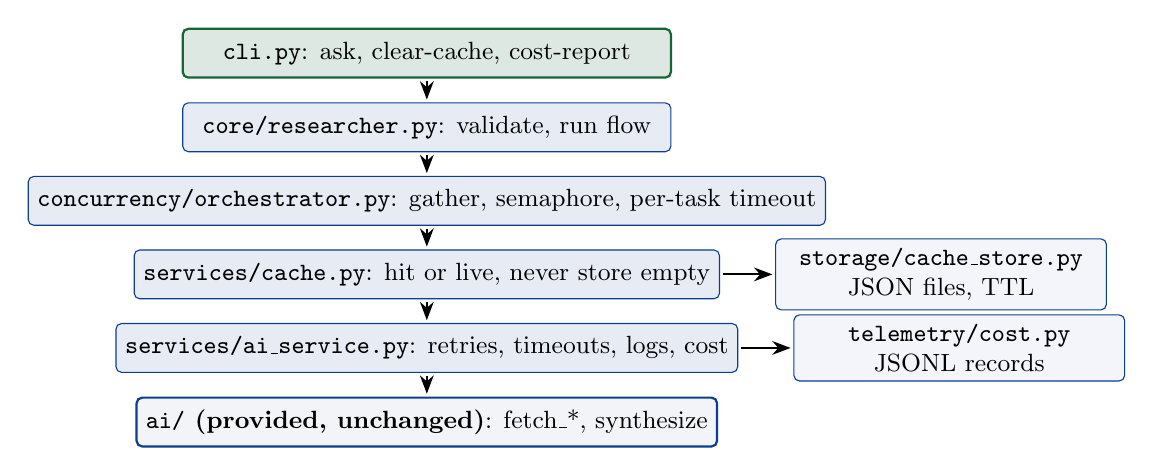
\begin{tikzpicture}[
  node distance=3mm,
  box/.style={draw,rounded corners=2pt,minimum width=6.2cm,minimum height=0.62cm,align=center,font=\small},
  aibox/.style={box,fill=soft,draw=accent,thick},
  sebox/.style={box,fill=accent!10,draw=accent},
  entry/.style={box,fill=ok!15,draw=ok,thick},
  side/.style={box,fill=accent!5,draw=accent,minimum width=4.2cm},
  arrow/.style={-Stealth,thick,shorten <=1pt,shorten >=1pt}
]
  \node[entry] (cli) {\texttt{cli.py}: ask, clear-cache, cost-report};
  \node[sebox,below=of cli] (core) {\texttt{core/researcher.py}: validate, run flow};
  \node[sebox,below=of core] (orch) {\texttt{concurrency/orchestrator.py}: gather, semaphore, per-task timeout};
  \node[sebox,below=of orch] (cache) {\texttt{services/cache.py}: hit or live, never store empty};
  \node[sebox,below=of cache] (svc) {\texttt{services/ai\_service.py}: retries, timeouts, logs, cost};
  \node[aibox,below=of svc] (ai) {\textbf{\texttt{ai/} (provided, unchanged)}: fetch\_*, synthesize};
  \node[side,right=0.7cm of cache] (store) {\texttt{storage/cache\_store.py}\\ JSON files, TTL};
  \node[side,right=0.7cm of svc] (cost) {\texttt{telemetry/cost.py}\\ JSONL records};
  \draw[arrow] (cli) -- (core);
  \draw[arrow] (core) -- (orch);
  \draw[arrow] (orch) -- (cache);
  \draw[arrow] (cache) -- (svc);
  \draw[arrow] (svc) -- (ai);
  \draw[arrow] (cache) -- (store);
  \draw[arrow] (svc) -- (cost);
\end{tikzpicture}
\end{center}

Exactly one module imports the \texttt{ai} package: \texttt{services/ai\_service.py}. Four call sites cross that boundary (the three fetchers plus \texttt{synthesize}). Exactly one module crosses the storage boundary: the cache facade, through \texttt{CacheStore.get} and \texttt{put}. Swapping the LLM provider changes one environment variable and zero source files. The synthesis path bypasses the cache and the orchestrator by design: \texttt{Researcher} calls \texttt{AIService.synthesize} directly, because an LLM answer depends on the fetched sources and is not a cacheable, per-source artefact.

\textbf{Module-by-module summary:}
\begin{itemize}[topsep=2pt,itemsep=1pt]
  \item \texttt{config.py} -- pydantic-settings model; 17 typed fields with validators, cached by \texttt{lru\_cache}.
  \item \texttt{models.py} -- \texttt{ResearchSession}: question, sources, answer, duration, per-source cache hits, failed sources.
  \item \texttt{storage/cache\_store.py} -- one JSON file per (source, canonicalised query), TTL-aware, corruption-tolerant.
  \item \texttt{telemetry/cost.py} -- appends one JSONL record per LLM call; summarised by \texttt{cost-report}.
  \item \texttt{services/ai\_service.py} -- tenacity retries, the synthesize thread-plus-timeout, structured logs, cost recording.
  \item \texttt{services/cache.py} -- cache facade returning \texttt{FetchResult(sources, cache\_hit)}; never stores empty lists.
  \item \texttt{services/failover.py} -- \texttt{FailoverLLM}, an \texttt{LLMProvider} that tries a configured chain of providers.
  \item \texttt{concurrency/orchestrator.py} -- the parallel fan-out with per-task isolation.
  \item \texttt{core/researcher.py} -- validate, fetch, synthesise, package.
  \item \texttt{cli.py} -- click commands, UTF-8 console setup, output rendering.
\end{itemize}

\subsection{OOP design \& key abstractions}

The provided \texttt{ai/providers/base.py} defines the abstract \texttt{LLMProvider} with three concrete subclasses selected by a factory. Our own use of inheritance plugs into exactly that seam: \texttt{FailoverLLM} subclasses \texttt{LLMProvider}, which is what lets \texttt{ai.synthesize(llm=...)} accept a failover chain without the provided package knowing failover exists.

\begin{lstlisting}[style=python,firstnumber=1]
class FailoverLLM(LLMProvider):
    """Tries each configured provider in order until one answers."""

    def __init__(self, factories: Sequence[tuple[str, ProviderFactory]]) -> None:
        if not factories:
            raise ValueError("at least one provider factory is required")
        self._factories = list(factories)
        self._instances: dict[str, LLMProvider] = {}
\end{lstlisting}

Providers are built lazily from factories, so the fallback SDK and API key are only needed if the primary actually fails. Everywhere else we use composition: \texttt{CachedAIService} holds an \texttt{AIService} and a \texttt{CacheStore}; the orchestrator holds the cached service; \texttt{Researcher} holds the orchestrator. If asked why these are not abstract base classes: each of those roles has exactly one implementation at runtime, so an ABC would add indirection without reuse. The failover chain is the one place where polymorphism earns its keep, and there we inherit.

\subsection{Data flow across module boundaries}

Typed values cross every boundary: \texttt{Settings} (configuration), \texttt{Source} and \texttt{AnswerWithCitations} (reused from \texttt{ai/}), \texttt{FetchResult} and \texttt{SourceResult} and \texttt{FetchOutcome} (frozen dataclasses inside the fetch path), and \texttt{ResearchSession} (returned to the CLI). No naked dictionaries flow between modules; the only dicts in play are the \texttt{cache\_hits} map inside \texttt{ResearchSession} and the JSON payloads at the storage boundary, where JSON is the point. We wrapped the provided models in \texttt{ResearchSession} exactly when SE-layer concerns appeared (timing, cache state, failure list) that do not belong to the AI module.

One deliberate detail: cache-hit information travels in return values rather than in shared mutable state on the service object, so two concurrent asks against the same service cannot interleave their bookkeeping.

% HABIL-BLOK-A: Section 3 (Concurrency & Performance) PR-12-de buraya elave olunacaq

\section{Robustness \& Error Handling}\label{sec:robustness}

\subsection{Wrapping the AI module}

Every \texttt{ai.*} call goes through \texttt{AIService}. Retries: tenacity, \texttt{retry\_if\_exception\_type(ProviderError)}, three attempts, exponential backoff between 1\,s and 8\,s, with a WARNING log before each sleep. Anything that is not a \texttt{ProviderError}, such as a \texttt{ValueError} from bad input, is a programmer error and is deliberately not retried; a unit test pins this distinction. Timeouts exist at two levels: each source fetch runs inside its own \texttt{asyncio.timeout} window (default 15\,s) owned by the orchestrator, and the blocking \texttt{ai.synthesize} call runs in a worker thread bounded by \texttt{asyncio.wait\_for} (default 60\,s). On synthesis timeout the caller gets a clean \texttt{ProviderError}; the abandoned worker thread finishes in the background, an accepted trade-off for a short-lived CLI process, and the docstring says so.

Logging is structured key=value text: \texttt{fetch\_start}/\texttt{fetch\_done} with source and result count at INFO, \texttt{source\_timeout}/\texttt{source\_failed} and retry notices at WARNING. No API key or payload is ever logged.

\subsection{Failure-mode analysis (one concrete incident)}

The incident we designed for arrived on its own. During a live run on July 20, Gemini returned HTTP 503 (\texttt{"This model is currently experiencing high demand"}) on the first synthesis attempt, again on the second, and succeeded on the third. The log shows the policy working exactly as written:

\begin{lstlisting}[style=python,language=bash,numbers=none,basicstyle=\ttfamily\footnotesize]
13:36:49 WARNING Retrying in 1 seconds as it raised ProviderError:
                 Gemini call failed: 503 UNAVAILABLE ...
13:36:52 WARNING Retrying in 2 seconds as it raised ProviderError:
                 Gemini call failed: 503 UNAVAILABLE ...
13:36:56 INFO    synthesize_done n_citations=2
\end{lstlisting}

The user saw a 13\,s answer instead of a crash. The same class of failure is pinned by unit tests on the fetch path: \texttt{test\_one\_source\_timeout\_does\_not\_block\_others} injects a 1\,s delay into a fake Wikipedia fetcher under a 0.05\,s timeout and asserts that arXiv and web still deliver, with \texttt{failed == ["wikipedia"]} surfaced to the user as a note under the answer. Writing that test drove the design: the first sketch let the timeout exception propagate through \texttt{gather} and cancel the batch; converting failures into structured \texttt{SourceResult} values is what made per-source isolation real.

A second real-world failure worth recording: on Windows the default console encoding (cp1252) crashed the first time Gemini emitted a Unicode arrow in an answer. The CLI now reconfigures stdout and stderr to UTF-8 before printing anything.

\subsection{Input validation}

\begin{itemize}[topsep=2pt,itemsep=1pt]
  \item \textbf{CLI.} Empty or whitespace-only questions raise \texttt{QuestionValidationError}, exit code 2. Questions over \texttt{MAX\_QUESTION\_LENGTH} (default 500) likewise. A 50\,000-character question is rejected before any network call. \texttt{--sources} values outside \{wiki, wikipedia, arxiv, web\} raise a \texttt{click.UsageError}.
  \item \textbf{Environment.} \texttt{Settings} validators reject an unknown \texttt{LOG\_LEVEL}, non-positive integers (\texttt{MAX\_PARALLEL=0}), and non-positive timeouts at startup, naming the offending field.
  \item \textbf{Cache files.} A corrupted JSON cache entry is logged at WARNING and treated as a miss, never a crash. Cache filenames are derived from a SHA-256 digest of the canonicalised query, so user input cannot traverse the cache directory.
  \item \textbf{Model output.} Out-of-range citation indices are dropped by the provided synthesizer; unexpected fields on our own models are rejected by \texttt{extra="forbid"}.
\end{itemize}

\section{Storage \& Caching}\label{sec:storage}

\subsection{Schema}

There is no relational schema; the cache is a flat directory of JSON files, one per (source, query) pair, named \texttt{\{source\}\_\{sha256[:24]\}.json} where the digest covers \texttt{source::canonicalised\_query}. Each file holds:

\begin{lstlisting}[style=python,language=bash,numbers=none,basicstyle=\ttfamily\small]
{
  "stored_at": 1784543740.29,     # POSIX timestamp at write time
  "value": [                      # list[Source.model_dump()]
    {"title": "...", "url": "...", "snippet": "...", "origin": "arxiv"}
  ]
}
\end{lstlisting}

The live provider is the source of truth; the cache is a derived view invalidated purely by age (\texttt{CACHE\_TTL\_SECONDS}, default 24\,h). If a future \texttt{ai/} upgrade changed the \texttt{Source} schema, re-validation through \texttt{Source(**item)} on read would fail loudly and the entry would be refetched. Cost telemetry uses the same directory: an append-only \texttt{costs.jsonl}, one record per LLM call.

\subsection{Caching policy}

We cache the per-source \texttt{list[Source]}, keyed by canonicalised query (lower-cased, trimmed, whitespace-collapsed), so \texttt{"What is X?"} and \texttt{"what  is x?"} share an entry. \texttt{--no-cache} bypasses both read and write. Two policy decisions matter. First, \emph{empty results are never cached}: an empty list usually means the source had a bad moment, or the question does not match a Wikipedia title, and remembering that for 24 hours would keep serving nothing after the source recovers. Second, the hit/miss state of every source is returned to the user on every ask (\texttt{cache: wikipedia=miss, arxiv=hit, ...}), which turned out to be the single most useful debugging signal in development. Measured behaviour on a repeated ask: arXiv and web hit; Wikipedia misses again exactly when its first response was empty, which is the no-negative-caching rule doing its job.

% HABIL-BLOK-B: Section 6-9, Tools, References ve Appendix PR-12-de buraya elave olunacaq

\vspace{1em}\hrule\vspace{0.6em}
\noindent\small\textit{End of report --- thank you for reading.}

\end{document}